
\documentclass[12pt]{article}


%%% PACKAGES

\usepackage[pdftex]{graphicx}

\usepackage{hyperref}
\usepackage{bibentry} %to use intext full bibliography entries instead of citations.  You will need a separate BibTex database for this to work.  See http://cst.usc.edu/services/tel/grants/legrants.html for details on this package.
\usepackage{booktabs} % for much better looking tables
\usepackage{array} % for better arrays (eg matrices) in maths
\usepackage{paralist} % very flexible & customisable lists (eg. enumerate/itemize, etc.)
%\usepackage{verbatim} % adds environment for commenting out blocks of text & for better verbatim
%\usepackage{subfigure} % make it possible to include more than one captioned figure/table in a single float


\usepackage{caption}

\usepackage{color}

%%% PAGE DIMENSIONS
\usepackage{geometry} % to change the page dimensions. Read ftp://ftp.tex.ac.uk/tex-archive/macros/latex/contrib/geometry/geometry.pdf for detailed page layout information 
\geometry{margin=1in} % for example, change the margins to 1 inches all round
%\geometry{landscape} % set up the page for landscape
% 

%%% HEADERS & FOOTERS
\usepackage{fancyhdr} % This should be set AFTER setting up the page geometry
\pagestyle{fancy} % options: empty , plain , fancy
\renewcommand{\headrulewidth}{0.4pt} % customise the layout...
%\lhead{}\chead{}\rhead{}
%\lfoot{}\cfoot{\thepage}\rfoot{}f

%\rfoot{\footnotesize SIR 330}
\rhead{\footnotesize BME 3300 Lab 1}
\renewcommand\footrulewidth{0pt}


%%% SECTION TITLE APPEARANCE
%\usepackage{sectsty}
%\allsectionsfont{\sffamily\mdseries\upshape} % (See the fntguide.pdf for font help)
% (This matches ConTeXt defaults)


%% END Article customise

%%% BEGIN DOCUMENT


\begin{document}


\thispagestyle{plain} %alternatively specify empty to get no footer on first page.  This is part of the fancyhdr package


\nobibliography{MasterBib} %this specifies the BibTex directory that stores your desired bibliography entries.  It has to come before any \bibentry lines are invoked

\bibliographystyle{apalike} %be careful here, there is only a few styles that will run


%\tableofcontents
\begin{center}
\bigskip

\textbf{BME 3300 Lab 1: Introduction to LabVIEW and Tools of the Trade} \medskip

\end{center}

\noindent In the first half of this lab you will learn how to use LabView, which will be used in subsequent labs and in many of your projects. 
In the second half you will get some hands-on experience with circuit building.

\bigskip

\noindent\textbf{Part I: Introduction to LabView}

\begin{enumerate}[1.]
	\item Go through chapters 1 to 4 (stop at page 4--6) of the LabVIEW program tutorial as outlined below. Each chapter should take between 15-20 min to complete.
	\begin{enumerate}[i.]
		\item Open LabVIEW 2014. An automatic initial Start Up menu appears.
		\item Select the \textbf{Getting Started with LabVIEW} option from the right menu pane. If this menu does not appear, access the pdf manual directly at \url{http://www.ni.com/pdf/manuals/373427j.pdf}. 
		Note that this is a manual for a previous version of LabView, so we give some corrections to it for LabView 2014 as follows: 
			\begin{itemize}
				\item Chapter 1, `Opening a new VI from template': The referenced VI is found in: {\bf{ VI $>>$ From Template $>>$ Simulated $>>$ Generate and Display}}
				\item Chapter 3, `Analyzing and Saving a Signal': The template VI for this exercise is no longer in the LabView installation; please ask the TA for it.
				\item Chapter 4, `Creating an NI-DAQmx Task': 
					\begin{itemize}
						\item You will need to use a BNC cable to connect the DAQ function generator to the chosen input channel on your DAQ board.
						\item Stop when you get to the ``Communicating with an Instrument'' section. 
						Skim the subsequent chapter sections for future reference. 
					\end{itemize}
			\end{itemize}
		Follow these tips or do a little searching around in LabView if something in the Manual doesn't make sense with the new LabView version - it can only help you later to become familiar with it!
		\item As this Getting Started manual details, the following 6 LabVIEW programs should
be generated. \underline{As you finish them, show them to the TA.}
		\begin{enumerate}[a.]
			\item Acquiring a Signal.vi
			\item Reduce Samples.vi
			\item Analysis.vi
			\item Warning Light.vi
			\item Save Data.vi
			\item Read Voltage.vi
		\end{enumerate}
	\end{enumerate}
	\item Let's get some more practice getting signals into your DAQ board. You will need BNC cables, your DAQ board, and your oscilloscope to complete this section. Create your own Data Acquisition module by doing the following:
	\begin{enumerate}[i.]
		\item In the Start Up screen, click on the \textbf{New...} button and open a \textbf{Blank VI}.
		\item Use the function generator on the National Instruments connector box to generate a sine wave in the 100-10 kHz range. Confirm that you see the sine wave on your oscilloscope.
		\item Use a BNC connector cable to input this sine wave into the analog input channel 0 (\textbf{ACH0}). Check to make sure that the switch above the input is on \textbf{BNC}, and that the switch below the channel is on \textbf{FS}.
		\item Right-click on the Block Diagram and choose \textbf{Programming} $\rightarrow$ \textbf{Structures} $\rightarrow$ \textbf{While Loop} to create a While Loop. Make it larger.
		\item Right click on the stop button in the lower right corner and select {\bf Create Control}. Notice how a stop button is now placed on the front panel.
		\item Again right-click on the Block Diagram and choose \textbf{Express} in the \textbf{Functions} menu. Then choose \textbf{Input} and insert a \textbf{DAQ} (\textbf{D}ata \textbf{A}c\textbf{Q}uisition) \textbf{Assistant} inside the while loop.
		\item In the \textbf{Create New...} window for the DAQ Assistant, click on the {\bf Acquire Signals} $\rightarrow$ \textbf{Analog Input} button.
		\item Then click on the \textbf{Voltage} button. Choose channel \textbf{ai0} under the \textbf{Supported Physical Channels} menu. Click \textbf{Finish}.
		\item In the \textbf{DAQ Assistant} window, make the voltage \textbf{Input Range} -10 V to +10 V. 
		Configure the assistant for \textbf{Continuous Sampling} and a 1 kHz sampling rate and 1000 {\bf Samples to Read}. Click \textbf{OK}. Your Block Diagram should now look similar to Fig. \ref{fig:1}.
	\end{enumerate}
	
	\begin{figure}[!h]
	\begin{center}
	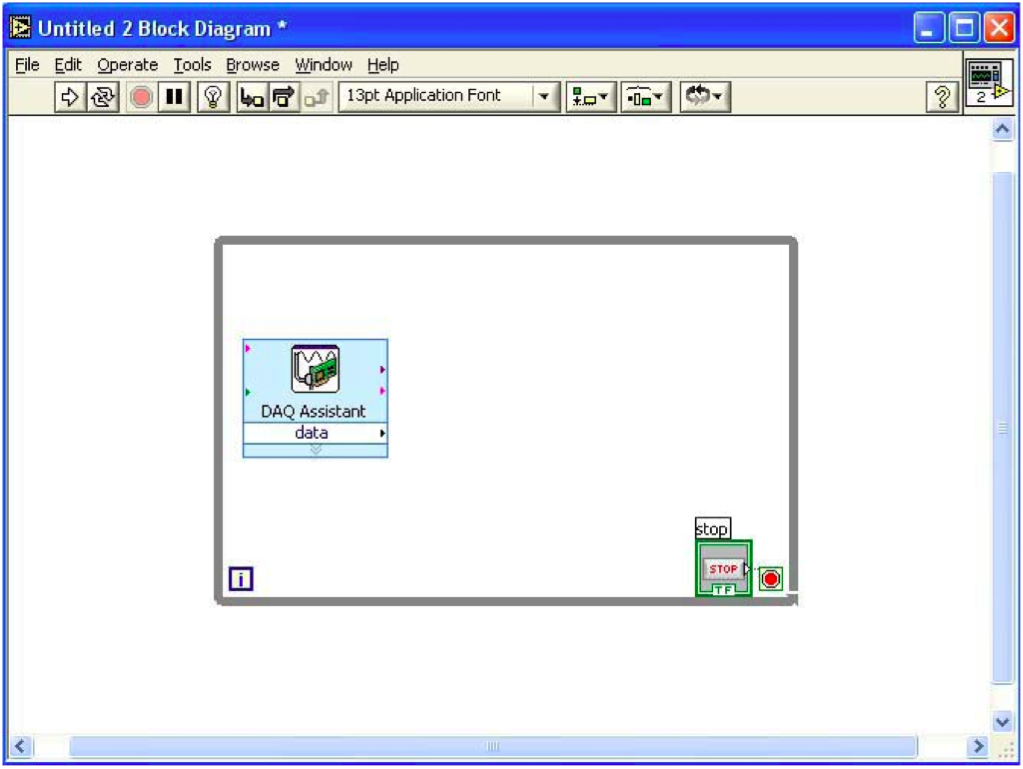
\includegraphics[width=0.75\textwidth,trim=0 0 0 0,clip=false]{lab1fig1.png}
	\caption{Block Diagram after completion of step 2.}
	\label{fig:1}
	\end{center}
	\end{figure}
	
	\item Create a Waveform Graph to display the signal generated by the function generator.
	\begin{enumerate}[i.] 
		\item Right-click on the \textbf{data} arrow of the DAQ Assistant, select \textbf{Create}, and then select
\textbf{Graph Indicator}. This creates a \textbf{Waveform Graph} to view the input from the LabVIEW function generator of the connector box. Your Block Diagram should now look similar to Fig. \ref{fig:2}.
		\item Run the program. Notice that the sine waves of the waveform are not clear, and that
adjusting the Amplitude and Frequency knobs on the connector box do not help to distinguish them.
		\item Stop the program and right-click on the DAQ Assistant. Select \textbf{Properties}. Reduce
the \textbf{Samples to Read} value to 200, and reduce the sampling frequency to 200 Hz.
		\item \textbf{Q}: Explain to the TA why the sine waves look more distinguishable now.
		\item Run the program again and observe the clearer waveform.
	\end{enumerate}
	
	\begin{figure}[!ht]
	\begin{center}
	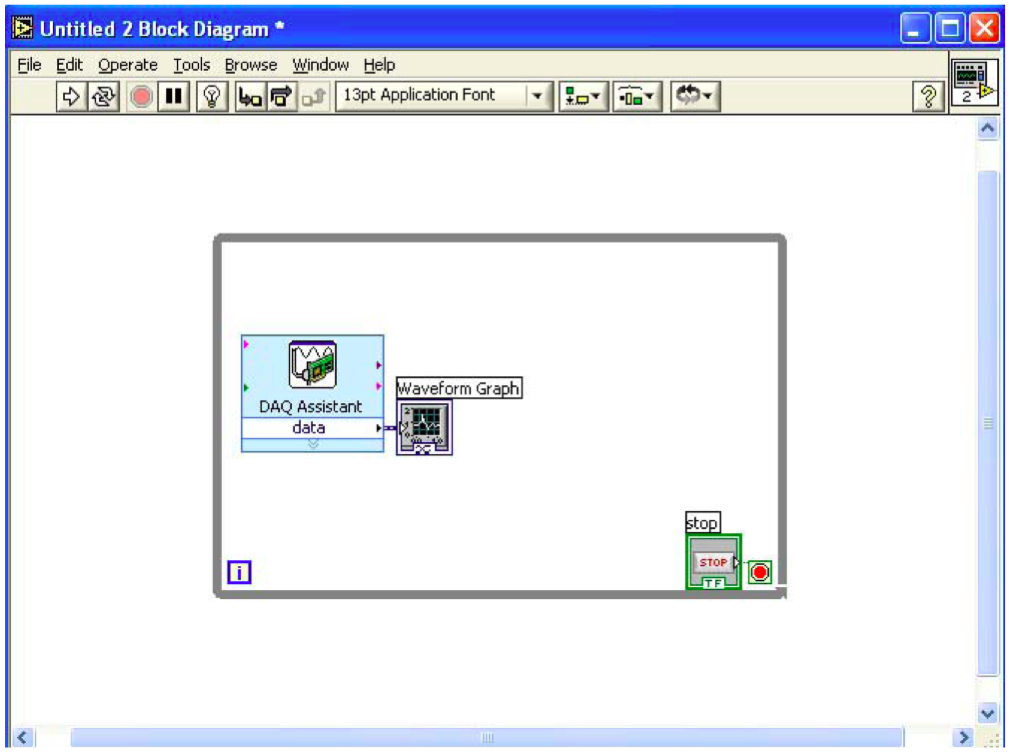
\includegraphics[width=0.75\textwidth,trim=0 0 0 0,clip=false]{lab1fig2.png}
	\caption{Block Diagram after completion of step 3.}
	\label{fig:2}
	\end{center}
	\end{figure}
	
	\item Insert a numeric indicator.
	\begin{enumerate}[i.]
		\item Right-click on the \textbf{data} arrow of the DAQ Assistant, select {\bf Create}, and then choose
{\bf Numeric Indicator}. Position it appropriately on the Front Panel, then run the program. Your Block Diagram should now look similar to Fig. \ref{fig:3}.
		\item \textbf{Q:} Tell the TA what values the numeric indicator displays.
	\end{enumerate}
	
	\begin{figure}[!ht]
	\begin{center}
	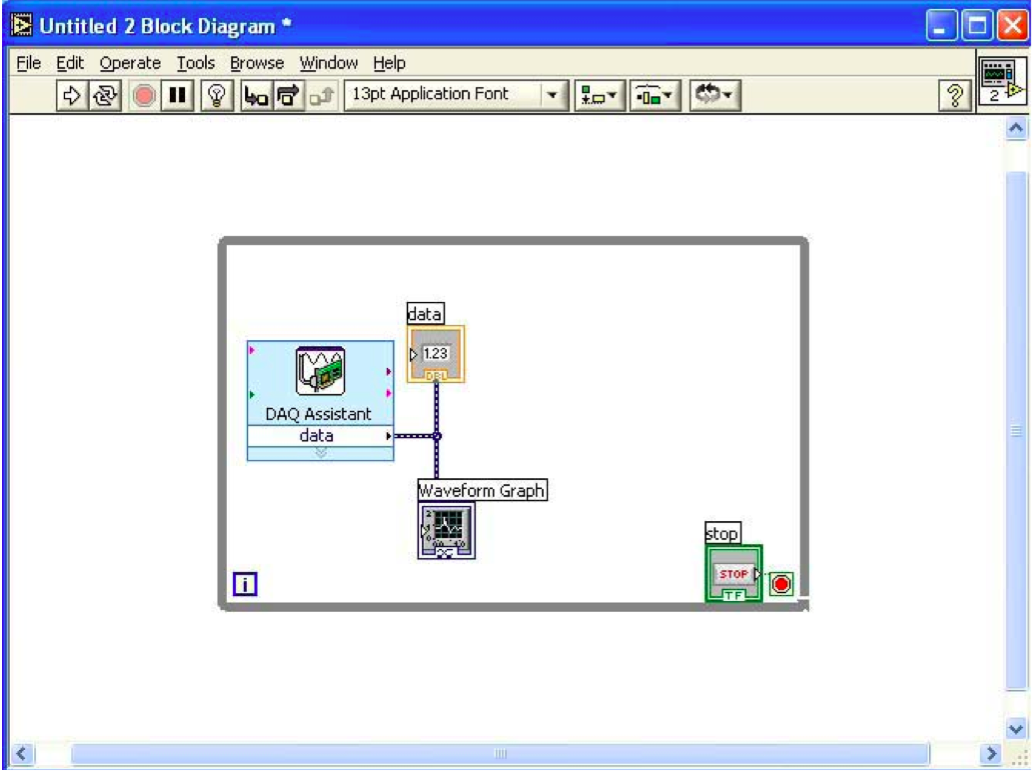
\includegraphics[width=0.75\textwidth,trim=0 0 0 0,clip=false]{lab1fig3.png}
	\caption{Block Diagram after completion of step 4.}
	\label{fig:3}
	\end{center}
	\end{figure}
	
	\item Insert a Boolean indicator.
	\begin{enumerate}[i.]
		\item Right-click on the Front Panel to reach the {\bf Controls} menu, choose {\bf LEDs}, and then
{\bf Round LED}. Appropriately position the LED on the Front Panel.
		\item On the Block Diagram, right-click to {\bf Programming} $\rightarrow$ {\bf Comparison} $\rightarrow$ $\mathbf{\geq}$? to make this comparator.
		\item Wire the {\bf Numeric Indicator} terminal and the {\bf X-terminal} of the comparator together.
		\item Right-click on the Y-terminal of the comparator, select Create, and then choose
Control.
		\item Wire the {\bf comparator output} to the {\bf LED input}. Your Block Diagram should now look similar to Fig. \ref{fig:4}.
		\item Run the program.
		\item {\bf Q:} Explain to the TA what mechanism makes the LED turn on and off.
	\end{enumerate}
	
	\begin{figure}[!ht]
	\begin{center}
	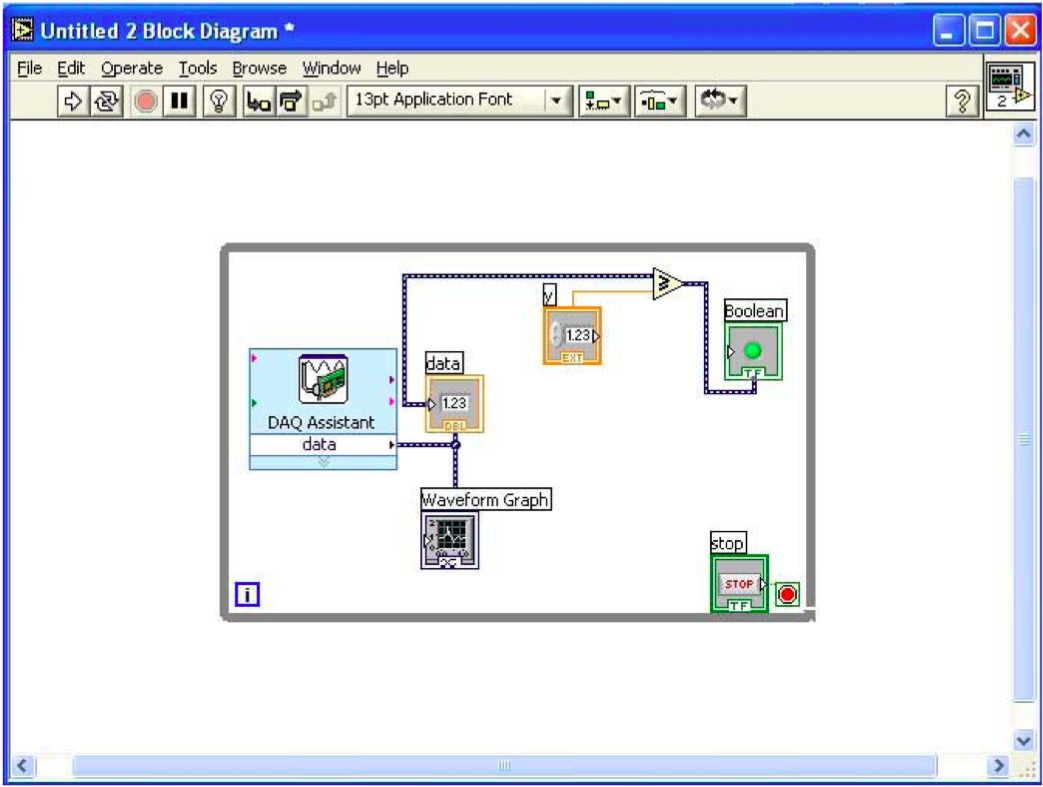
\includegraphics[width=0.75\textwidth,trim=0 0 0 0,clip=false]{lab1fig4.png}
	\caption{Block Diagram after completion of step 5.}
	\label{fig:4}
	\end{center}
	\end{figure}
	
	\item Write acquired data to a file.
	\begin{enumerate}[i.]
		\item Right-click on the Block Diagram to select {\bf Programming} $\rightarrow$ {\bf File I/O} $\rightarrow$ {\bf Write Meas File}.
		\item In the {\bf Configure Write LabVIEW Measurement File} window, set the file name to ``SineWaveProperties.lvm''. Set the file location to the `BME 3300 Labs' folder on the Desktop.
		\item Wire the data output of the DAQ Assistant to the Signals input of the Write LabVIEW Measurement File Express. Your Block Diagram should now look similar to Fig. \ref{fig:5}.
		\item Save this program as SineWavesProperties.vi. Take a screen shot of the front panel and block diagram (using the Windows Snipping Tool under {\bf Programs} $\rightarrow$ {\bf Accessories} $\rightarrow$ {\bf Snipping Tool}) and save it with a .jpg extension in the 3300 folder (you can also use Paint for this). \underline{Show the jpeg image to the TA.}
		\item Open and view the output file ``SineWaveProperties.lvm'' generated by LabView.
	\end{enumerate}
	
	\begin{figure}[!ht]
	\begin{center}
	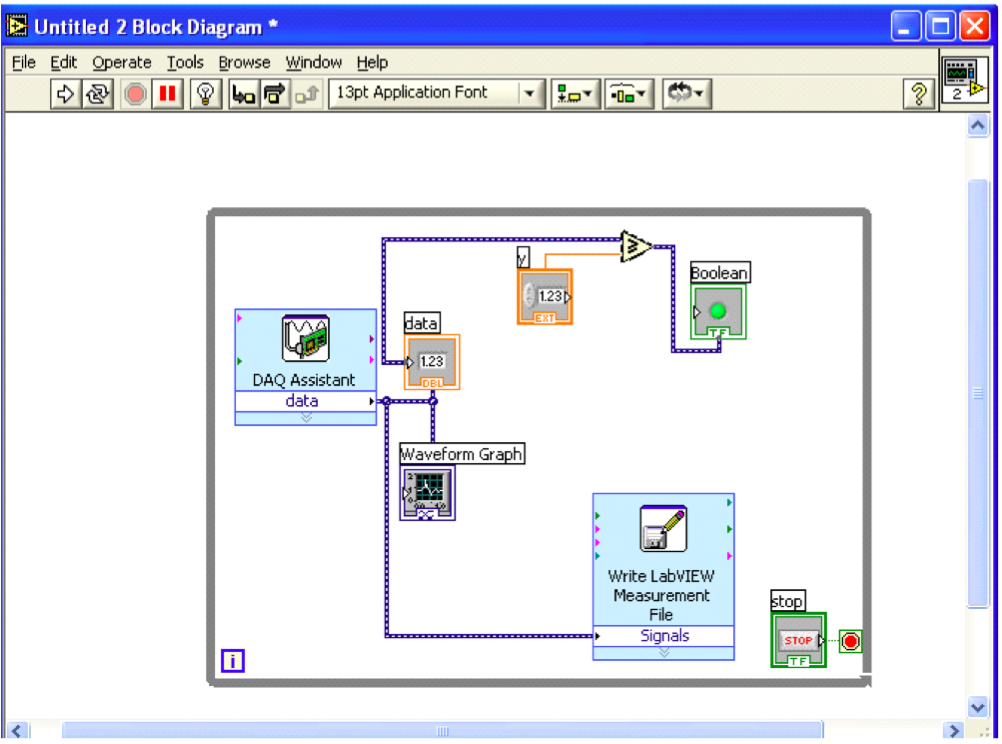
\includegraphics[width=0.75\textwidth,trim=0 0 0 0,clip=false]{lab1fig5.png}
	\caption{Block Diagram after completion of step 6.}
	\label{fig:5}
	\end{center}
	\end{figure}
	
\end{enumerate}

\newpage

\noindent\textbf{Part II: Tools of the Trade}

\noindent In this part of the lab, we're going to cover some basics, essential to any electronic construction project. Some of you may know most of these, but others may not, or you may not know it as well as you think.

\begin{enumerate}[1.]%[leftmargin=0cm,itemindent=.5cm,label=\Alph*.,labelwidth=\itemindent,labelsep=0cm,align=left]%[A.]
\item{\bf Wire}

What could be more simple than wire? You use it to allow current to flow from one point to another. However, while wire is fundamentally a very straightforward idea, nobody teaches it anymore. I have seen a student project involving 6 high-end DSP chips fail, not because the student didnÕt understand the DSP chips but because they didn't understand wire.

\par With very few exceptions wire is made out of copper, an excellent conductor because it has only 1 electron in its outer shell. When copper molecules bond to form metallic copper, that electron is free to move as an electron cloud, allowing easy conduction.
The resistivity of copper is 1.72$\times$10$^{-8}$ $\Omega$ per cubic meter.

\par Since resistance equals (resistivity $\times$ length)/cross sectional area and most wire is extruded as a cylinder giving it a circular cross-section, 
wire resistance = length $\times$ resistivity/ $\pi$(D/2)$^2$ (D = diameter) which for copper wire is 2.19$\times10^{-8}$ ohms per meter /D$^2$. 
As the diameter goes up the resistance goes down. 
Lower resistance means less energy lost as heat. 
For historic reasons, wire diameter is listed as gauge numbers which have the unfortunate problem of increasing as diameter decreases. 
(Unfortunate in that the inverse relationship makes it difficult to remember) 
This is shown below:
\begin{center}
\begin{tabular}[!h]{|c|c|}\hline
{\bf Gauge} & {\bf Diameter (mm)} \\ \hline
6 & 4.115 \\ \hline
12 & 2.05 \\ \hline
16 & 1.29 \\ \hline
22 & 0.644 \\ \hline
30 & 0.255 \\ \hline
\end{tabular}
\end{center}
\par Lamp cord (occasionally called zip cord) is the size wire you see providing power to small appliances such as clock radios and, well, lamps. 
Lamp cord is 16 gage wire which means 1000 meter length of it would have a 13.1 $\Omega$ resistance. 
Since a 100 watt bulb draws a little less than 1 amp of current, obviously a meter or so of lamp cord can handle a couple of amps of current relatively easily.

\par The wire you use in breadboards is 22 gauge wire and it differs from lamp cord, not only in size but it is solid core wire as opposed to lamp cord which is {\it stranded}. 
Stranded wire is much more flexible than solid wire of the same cross section, so it is easier to use. 
However, wire gauge are set by the outside diameter not the total cross sectional area. 
Because it is impossible to pack strands of wire perfectly tightly, stranded wire has slightly less current carrying capacity than solid wire of the same gauge. 
This is compounded if you mechanically distress the wire. Some strands may break, reducing the effective cross sectional area. 
Because of this all house wiring in the walls should be solid core. 
Finally, the smallest wire you might use in this lab is wire-wrap wire (30 gauge). 

\par Imagine the following circuit:

%\begin{figure}[!h]
\begin{center}
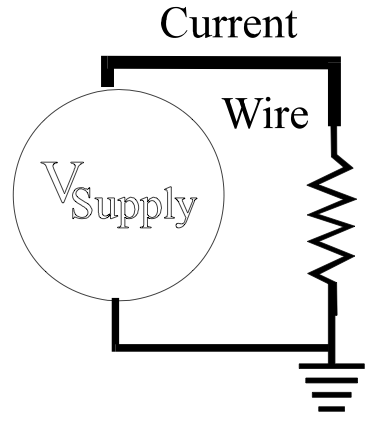
\includegraphics[width=0.25\textwidth,trim=0 0 0 0,clip=false]{lab2fig1.png}
%\caption{Block Diagram after completion of step 2.}
%\label{fig:1}
\end{center}
%\end{figure}

Let's say we have 0.2 amps going through 1 meter of wire. If the wire is zip
cord then we have 34 microwatts of power dissipated in the wire. 
If it is 22 gauge hook-up wire we have 557 microwatts of power dissipated in the wire. 
If itÕs wirewrap wire we have 22.7 MILLIwatts of power dissipated in the wirewrap wire. 
So just by wire gauge alone we can have almost a 1000 fold increase in the power dissipated in the wire. 
Since that power is dissipated as heat, wire gauge matters.

\par Take Home Tip: When you are building a circuit using wirewrap keep the distance (in terms of wire wrap wire) between your power supply connections and each chip as
short as possible to minimize power loss in the wires. 
This is especially important with you ground connections. Use star patterns instead of chains as shown below.

\begin{figure}[!ht]
\begin{center}
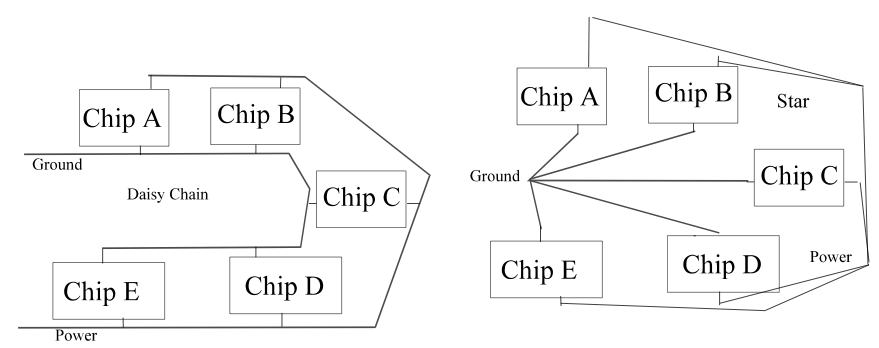
\includegraphics[width=\textwidth,trim=0 0 0 0,clip=false]{lab2fig2.png}
%\caption*{}
%\label{fig:1}
\end{center}
\end{figure}

You may want to construct ``local'' power supplies and ground connections using larger diameter wire in order to prevent too much current from moving down wire wrap wire.

{\bf Cables}\\
An electrical connector with one conductor in it is a wire, if it has more than one conductor, it is a cable. The most often used cable is coaxial cable (called coax). Coax has a central conductor and a metallic braid that form two conductors. (See Below). The general use is that you send your signal down the central conductor and apply a ground to the braid. The advantage of this arrangement is that stray signals falling on the coax are absorbed by the braid and therefore do not end up on central conductor to interfere with your signal. There are two disadvantages to coax. First, it is rather difficult to work with, and to make good connections without
shorting the braid to the central connector. Second, the surface of the central conductor is separated from the braid by insulation. So you have two conducting surfaces, parallel to each other separated by a non-conductor or dielectric. Sounds like a capacitor to me. This capacitance can distort waveforms traveling down the central conductor.

\begin{figure}[!ht]
\begin{center}
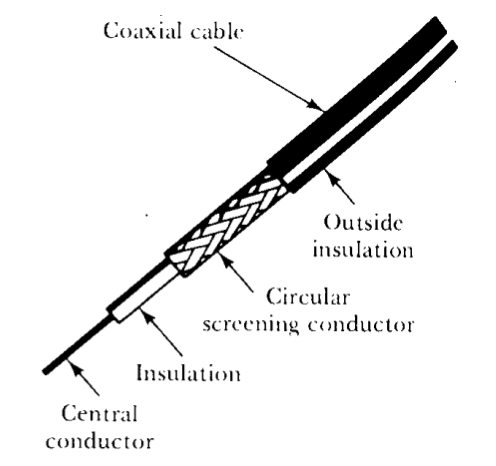
\includegraphics[width=0.33\textwidth,trim=0 0 0 0,clip=false]{lab2fig3.png}
\caption*{Coax cable.}
%\label{fig:1}
\end{center}
\end{figure}

{\bf Connections}\\
Now that you understand about wire and cable, you have to put it to use. 
As stated earlier the purpose of wire and cables
is to provide a path for current flow from one point to another. 
To accomplish this we have to anchor the wire at those two points. 
This requires mechanical stability while maintaining electrical connections. 
It would also be a boon if the connections may be relatively easily undone for revision or repair.

\par Obviously the simplest way to connect two wires is to twist them together. 
While easy to revise or repair, this technique is neither mechanically nor electrically stable. 
The mechanical and electrical stability of two twisted wires may be improved by soldering the wires together. 
Solder, an alloy of tin, lead, bismuth and other metals, melts at a much lower temperature than copper. 
Soldering is accomplished by heating the copper until it reaches the melting point of solder. 
The solder is applied to the copper and liquefies, where upon which it flows by reduction of surface tension to coat the copper. 
As the solder cools, the metal jacket formed holds the copper together. 
While solder is conductive, the primary connection should still be copper to copper.

%\par While solder solves some of the problems with simple twisting, it does so at the cost of increased complexity in revising or repairing a join. 
%The wire has to be de-soldered changed and resoldered. 
%It is also possible to make a solder joint which looks fine but has little copper-to-copper connections which leads to failure. 
%In the late 1930Õs an engineer named Uncas Whitaker came up with a new way to connect wires. 
%What Whitaker came up with was a ring connector which could be mechanically crimped onto the end of a wire as shown here.
%
%\par This meant that to connect two wires together you just ran a bolt through the hole and screwed a nut onto the bolt. To add another wire or replace a present one, just unscrew the nut and add another ring. From this simple idea, Whitaker founded AMP industries. WhitakerÕs timing couldnÕt have been better. With the onset of World War II, the US and allies had to massively ramp up constructions of airplanes, ships , trucks and tanks. To have a connector system which was simple, rugged, flexible and could be correctly installed by minimally trained labor was a huge boon. AMP became one of the leading companies in the post-war boom. (As a sidelight, in 1975 Uncas Whitaker died and left \$100 million dollars to form the Whitaker Foundation, an organization which transformed Biomedical Engineering by providing grants for new BME faculty and to form BME departments).

{\it Quick Soldering Tutorial:}\\
Soldering is a fine art and takes practice. 
Here are some tips (most are from hackaday.com):
\begin{itemize}
  \item Be careful with the iron, the hot tip WILL give you 2nd degree burns and that's no fun.
  \item Don't breath in the solder
  \item More soldering tips can be found by Googling or asking the TA
\item Don't bake your bits. 
Passive components like resistors or small ceramic capacitors don't usually suffer any problems from being heated up, but you should still pay attention to how long you've been cooking them with your soldering iron. 
If you're having problems getting a solder joint just right, let the parts rest for a few minutes so they have a chance to cool off between soldering rounds.
\item Integrated circuits like logic chips are usually far more sensitive to heat and static than passive components. 
Sockets (below) are cheap insurance against blowing a chip.
\begin{figure}[!ht]
\begin{center}
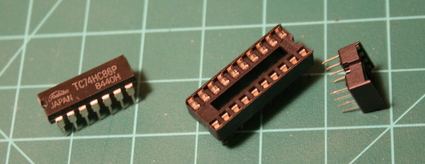
\includegraphics[width=0.33\textwidth,trim=0 0 0 0,clip=false]{sockets.png}
%\caption{Block Diagram after completion of step 2.}
%\label{fig:1}
\end{center}
\end{figure}
\item Do not melt the solder on the tip of the iron. 
Sometimes it's necessary to melt a small amount on the iron to facilitate heat transfer, 
but to achieve a good connection, you want the solder to melt and flow onto the component leads. 
So heat up the component with the iron just before applying solder.
\item Wipe solder and burn rosin off the iron by pulling the tip across your wet sponge or paper towel.
\item Nobody's perfect. 
Sometimes we need to remove a bad component or undo a mistake. 
Desoldering braid (or wick) works sort of like a sponge for excess solder.
\item To desolder something, just place the braid over the target and apply your soldering iron over the top (shown below). 
The heat should transfer through the braid and the melted solder will flow onto the the copper like oil though a wick. 
\begin{figure}[!ht]
\begin{center}
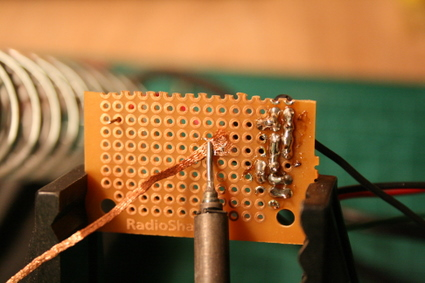
\includegraphics[width=0.5\textwidth,trim=0 0 0 0,clip=false]{wick.png}
\caption*{Desoldering with solder wick.}
%\label{fig:1}
\end{center}
\end{figure}
\end{itemize}

{\bf Task 1: Soldering}\\
Get a piece of perfboard, insert two pieces of wire-wrap wire through it, and twist and solder them together. 
To practice solder wicking, insert another piece of wire through the perfboard and melt some solder onto it. 
Then remove that solder with the iron and wick.
Next, get a piece of plated perfboard and stick a DIP chip into it. 
Make sure the leads stick out the plated side. 
Practice soldering each lead of the chip. 
Use enough solder to make a nick filled around the leads and fill in the hole, but not so much that it clumps up or shorts two leads together. 
If you get too much solder, use some wick to remove the excess. 
\underline{Solder a chip and show it to the TA.}
For a real challenge, use the wick or the desolder pump to remove all the solder and remove the chip from the board.
Give each person in your group a turn to practice these steps.

\begin{figure}[!ht]
\begin{center}
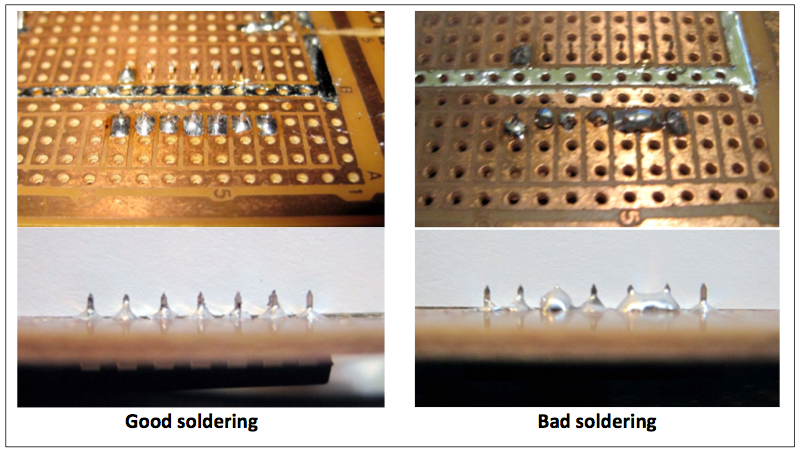
\includegraphics[width=\textwidth,trim=0 0 0 0,clip=false]{dipchipsolder.png}
\caption*{Soldering a DIP chip.}
%\label{fig:1}
\end{center}
\end{figure}

\par How about coax cable? 
Since the key to coax is the braiding surrounding the central conductor, you don't want to change that arrangement. 
The most common type of connector for coax is a BNC connector (I have no idea where the name comes from!) 
Here the outer shell is connected to the ground braid and the central conductor is connected to a pin in the middle of the connector.

\item{\bf Temporary Connectors (Switches)}
There are times when you want to interrupt current flow through a conductor (for example for 1996 Christmas, Coleco introduced a new Cabbage Patch doll which made a chewing motion when a spoon was placed in the dollÕs mouth. Unfortunately it made the same motions when a childÕs hair entered the dollÕs mouth. In a brilliant design move Coleco saved itself
\$0.35 per doll by not having an on-off switch. So
children were treated to the Daily Double Traumatic
Experience of: first having their new dolls chew their
hair like crazed weasels and then, second, having their
parents decapitate the dolls trying to turn it off.) To
interrupt the current flow with the connections we
covered above might require unsoldering some wires
(hardly convenient) or ripping a dollÕs head off. So
to interrupt the current flow, switches were invented.
The most basic switch is shown below.

\begin{figure}[!ht]
\begin{center}
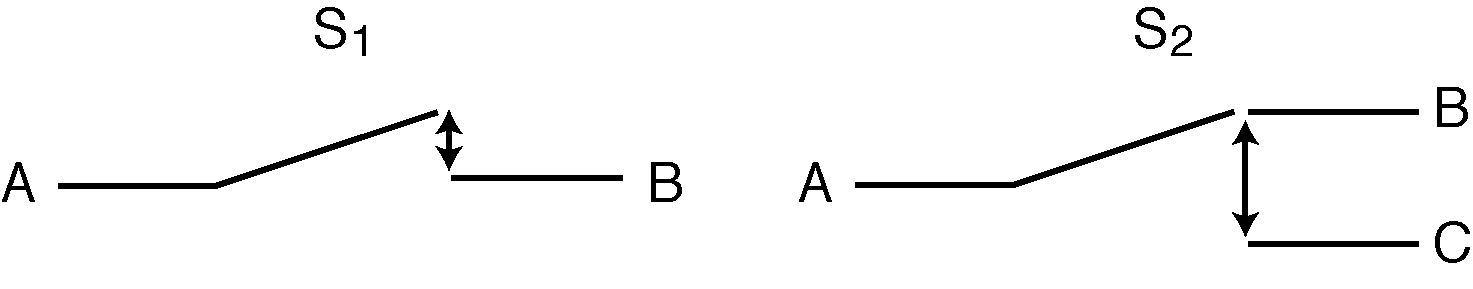
\includegraphics[width=0.66\textwidth,trim=0 0 0 0,clip=false]{lab2fig4.png}
\caption*{SPST and SPDT switches.}
%\label{fig:1}
\end{center}
\end{figure}

\par Switch S$_1$ allows A to be connected to B or not. 
When A connects to B the switch is closed or made. When A is not connected to B, S$_1$ is open or broken. 
Because S$_1$ controls a single conductor it is a single pole switch (this has nothing to do with a single pole filter). 
Because it can only make or break with 1 point it is a Single Throw switch. 
So S$_1$ is a Single Pole Single Throw (SPST) switch. 
S$_2$ is also a single pole switch, however, in S$_2$, A can connect to B or C. 
This makes it a Single Pole Double Throw switch (SPDT).

\begin{figure}[!ht]
\begin{center}
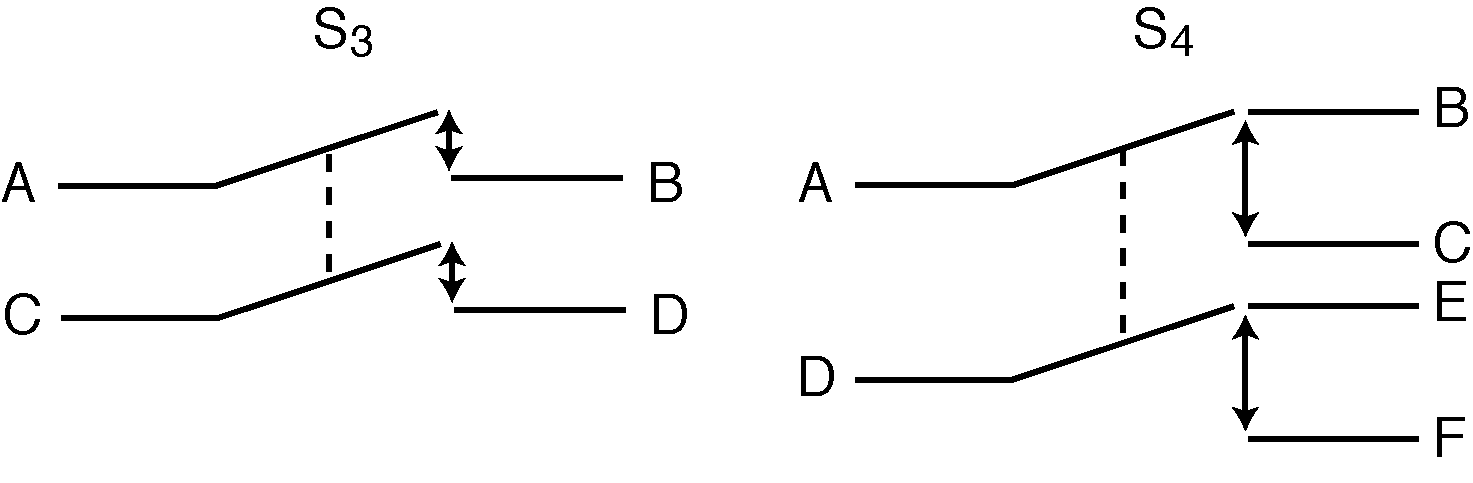
\includegraphics[width=0.66\textwidth,trim=0 0 0 0,clip=false]{lab2fig5.png}
\caption*{DPST and DPDT switches.}
%\label{fig:1}
\end{center}
\end{figure}

\par There are times when you want to control multiple connectors at the same time. 
That is, one switch makes or breaks multiple connectors simultaneously. 
These are shown in S$_3$ and S$_4$ above. 
S$_3$ is a Double Pole Single Throw (DPST) and S$_4$ is a Double Pole Double Throw. 
You should note that the (dashed-line) connection between poles is purely mechanical, no electrical connection exists.

\par There are times when you want to change the state of a switch (open from closed or closed from open) for only as long as the button is depressed. This is known as a momentary switch and they can be purchased as normally open or normally closed. Then when the switch is depressed they change state, returning to their normal state when the switch is released. (Kind of a Jekyll and Hyde thing - Depressed, Change State, After some time return to normal...)

\item{\bf Linear Components}\\
{\bf Resistors}\\
Resistors are like poor wires, they allow some current flow between points but they restrict the amount. Since EE112 you have been dealing with resistorÕs values, but there doesnÕt seem to be much coverage of their power ratings. We use $1/4$ watt resistors, 
which means that the current in amps squared times the resistance in ohms should be less than 0.25. 
In BME we tend to use very small currents ($<$20 millamps) so $1/4$ watt resistors are usually fine.

\par Resistor Color Codes: Resistors are color coded (see chart below). 
The first two stripes denote a 2 digit number (such as Yellow Violet for 47) and the third denotes an exponent of 10 to multiply the first two digits by. 
For example a Yellow Violet Red set of stripes would translate as 47$\times10^2$ or 4.7 k$\Omega$. 
The fourth stripe tells you the resistorÕs precision. Gold for 5\%, silver for 10\%. 
This you probably had in EE 213. 
What you have probably not been told is that when the manufacturer makes resistors they donÕt make a up a vat of 10000 5\% resistors. 
They make up a vat of resistive material and form resistors. 
Those resistors have their resistance measured by a machine which then paints them. 
If the value is within 5\% of a standard value (see below) it gets a gold stripe, if it is with 10\% it gets a silver stripe. 
As explained below, that covers all possible standard resistances. 
But think about it for a second. 
If you have silver banded resistors they are within 10\% of the standard but must be greater than 5\% in error or they would have gold bands,
meaning that they must be between 5-10\% off.

\begin{figure}[!ht]
\begin{center}
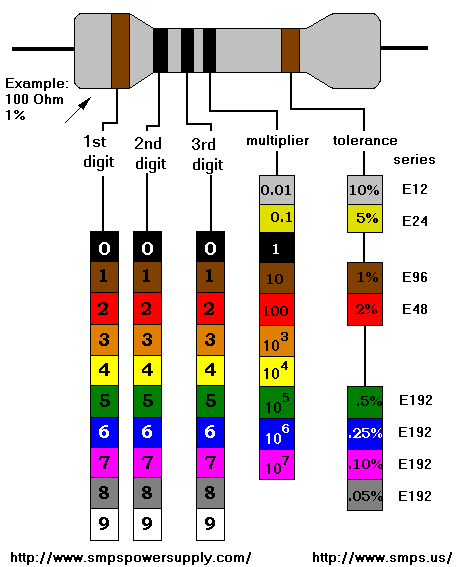
\includegraphics[width=0.66\textwidth,trim=0 0 0 0,clip=false]{colorcodes.png}
\caption*{Resistor color codes.}
%\label{fig:1}
\end{center}
\end{figure}

\par When you go looking for a resistor of a particular size, you may notice a rather odd spacing between standard resistor values. 
For example, in 10\% resistors from 1k ohms to 10k ohms the standard values are 1k, 1.2k, 1.5k, 1.8k, 2.2k, 2.7k, 3.3k, 3.9k, 4.7k. 5.6k, 6.8k and 8.2k. 
Why not 3.0k or 9.1k? 
Each of these values is roughly 20\% greater than the value below it. 
Therefore a $\pm$10\% range of a value covers most of the space between values.

{\bf Task 2: Resistor sorting}\\
Each group should get 10 resistors and put them in the appropriate resistor drawer, 
or lay them out with labels on a sheet of paper. 
Confirm the color code with your multimeter.

{\bf Capacitors}\\
Capacitors are formed by taking parallel plates of conducting material and placing a
nonconducting material (dielectric) between them. 
The area of the plate ($A$) times the
dielectric ($\epsilon$) divided by the thickness of the dielectric ($d$) gives the capacitance:
\begin{equation}
C = \frac{\epsilon A}{d} 
\end{equation}
The
dominant problem here is that the dielectric is a material property. It is a measure of
how much electric field can be applied before charge leaps from the one plate to another. 
You could increase capacitance by decreasing $d$ but that just shortens the gap that a charge would have to jump. 
So to make larger capacitances, you must increase $A$. 
If you make $A$ a flat plate, as shown below, it would get bulky and unusable pretty quickly. 
What is done to increase $A$ without making a huge device is to roll up the plates.

\begin{figure}[!ht]
\begin{center}
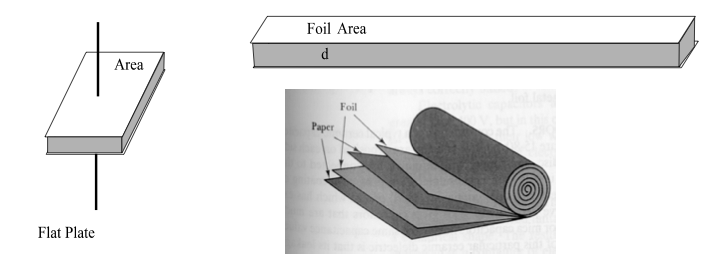
\includegraphics[width=\textwidth,trim=0 0 0 0,clip=false]{capconstruct.png}
\caption*{Capacitor construction}
%\label{fig:1}
\end{center}
\end{figure}

\par For some reason which eludes me, capacitor manufacturers have not standardized on a color code like resistor
manufacturers. 
So in the absence of any color code let me give you the Dr. Bob's Sure Fire Never Fail Capacitor Value Determination Method which is guaranteed to be
right at least 60\% of the time. 
If the capacitor is smaller than your thumbnail and the number on it is greater than 10, the capacitor is in picofarads ($10^{-12}$). 
Otherwise it is in microfarads ($10^{-6}$).
So if you see a small capacitor marked 103 it is a $10\times10^3$ picofarad (pronounced ``puff'') cap or $10^{-8}$ farads. 
In this lab we will use 20\% tolerance capacitors so the value you read on them should be considered a suggestion rather than an exact value.

\par Now there is one more complication to capacitors. (``Of course, I understood things so far'') 
The material that forms the dielectric is important for two reasons: dielectric value and dielectric breakdown voltage. 
Depending on the material and its intrinsic dielectric you can have large or small areas (and thus physical size). 
As you might guess, you can get smaller physical size for the same capacitance using exotic materials (polyethylene instead of paper as a dielectric) but at a higher cost. 
One other trick for increasing capacitance is to use aluminum plates and an electrolyte soaked gauze pad for a dielectric. 
The manufacturer then applies a DC voltage to the aluminum plates (positive on one side negative on the other) and a fine coating of aluminum oxide forms on the positive plate. 
This is the very thin dielectric and so you get high capacitance in a small size. 
These capacitors are called electrolytic capacitors, and are shown below. 
The problem with this is what happens if you reverse the voltage? 
The oxide wants to coat the other plate. 
The transition of this plating forms a gas and the capacitor could explode. 
Therefore when you buy an electrolytic cap, one terminal is marked ``+''. 
This terminal should always be kept more positive than the other.

\begin{figure}[!ht]
\begin{center}
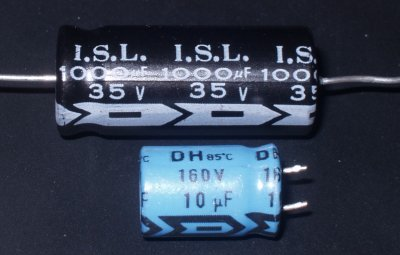
\includegraphics[width=0.33\textwidth,trim=0 0 0 0,clip=false]{ec.png}
\caption*{Electrolytic capacitors.}
%\label{fig:1}
\end{center}
\end{figure}

\par The second effect of the dielectric material is dielectric breakdown voltage. 
On a dry winter morning when you are shuffling around on the rug in your bunny slippers you are accumulating charge (expressed as a voltage) on your skin. 
When you find some victim, you sneak up on them and point with your finger, getting closer and closer until a spark jumps from you to some sensitive part of your victim's anatomy. 
Cackling wildly you escape having demonstrated both dielectric breakdown and a callous attitude to those around you. 
What happened? 
When faced with an electric field, a non-conductor (dry air in this case) resists current flow (a spark). 
However, if the field gets high enough, it can cause a temporary ionization allowing conduction until the voltage is removed. In the case of the Great Bunny Slipper Caper the voltage is removed by draining the charge from you to your victim. 
This can happen in capacitors. 
To prevent this problem capacitors are rated with a maximum DC voltage. 
If this voltage is exceeded, you can get dielectric breakdown and your capacitor becomes a short.

{\bf Task 3: Filter}\\
Now that you know about resistors and capacitors, you can build the filter circuit below on a breadboard.
If you've never used a breadboard before check out the diagram on the board for reference.
\textbf{Never attempt to solder anything onto the bread boards!}
Note that the exact values of the resistor and capacitor may change subject to parts availability.

\par Once the filter is built, connect the signal generator to the input, and the oscilloscope to the output. 
Set the signal generator to produce a low-frequency sinusoidal signal (10's of Hz), then set it to a very high-frequency signal (MHz). 
What kind of filter is this?
Using the oscilloscope, measure the 3 dB down frequency of this filter, 
by looking for the frequency at which the amplitude of the signal on the scope drops to $1/\sqrt{2} \approx 0.707$ of its maximum value.
We will see in class that the 3 dB down (or corner) frequency of this filter is:
\begin{equation}
f_c = \frac{1}{2\pi R C}.
\end{equation}
Does your measured frequency agree with the predicted one?
Do they agree? Why or why not?
Check the resistance of the resistor using the multimeter. 
Given this value and your measured corner frequency, what is your capacitance? 
How far off is that (in \%) from the labeled value?
\underline{Show the TA your circuit and your results.}
If you can't see a signal on the oscilloscope make sure it is on and that the BNC cable is plugged into the correct channel. Also try turning the amplitude/x/y position up and down to see if the signal appears.

\begin{figure}[!ht]
\begin{center}
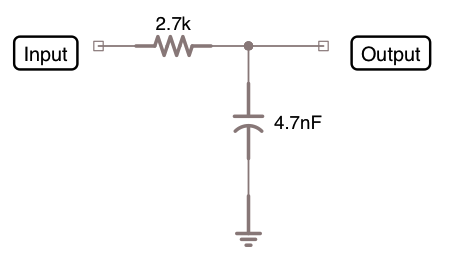
\includegraphics[width=0.5\textwidth,trim=0 0 0 0,clip=false]{lpf.png}
\caption*{Filter to build.}
%\label{fig:1}
\end{center}
\end{figure}

{\bf Inductors}\\
Inductors are difficult. 
They are resistive and capacitive, leading to all sorts of unexpected phenomena. 
The only real world advice I can give you is the following. 
Inductors tend to be labeled with their values, they also often have ranges of frequencies in which they act most like pure inductors. 
The lower the inductance the closer they are to acting purely as inductors.

\item{\bf Non-linear Components: Semiconductors}\\
The response of resistors, inductors and capacitors to both positive and negative currents and voltages is governed by a single linear equation, 
characteristic to the circuit element. 
However, there are times when we don't want linear responses.

{\bf Diodes}\\
Diodes serve as one-way valves for current. 
They're drawn as below. If $V_A$ $>$ $V_B$ then current wants 
to flow in the direction shown by I. 
The diode will allow this and enough current will flow so that $V_A$ is only slightly greater than $V_B$.
I'll get to that later.
\begin{figure}[!ht]
\begin{center}
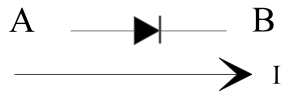
\includegraphics[width=0.33\textwidth,trim=0 0 0 0,clip=false]{diode1.png}
%\caption*{Filter to build.}
%\label{fig:1}
\end{center}
\end{figure}
\par If $V_A < V_B$ then current wants to flow in the direction shown by the squiggly arrow. 
The diode does not allow this to happen.
\begin{figure}[!ht]
\begin{center}
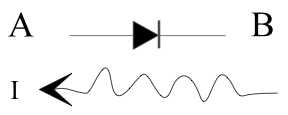
\includegraphics[width=0.33\textwidth,trim=0 0 0 0,clip=false]{diode2.png}
%\caption*{Filter to build.}
%\label{fig:1}
\end{center}
\end{figure}
\par It is this ``current valve'' behavior that allows us to use diodes to select parts of bipolar processes such as sine waves and act on them independently. 
If we place a sinusoid into the circuit below, during the positive half of the sinusoid the diode is open and current flows through the resistor. 
How much current? 
Enough so that $V_{OUT}$ is equal to $V_{IN}$ minus that to-be-named later ``slightly greater''.
On the negative half of the cycle the current would like to flow from ground back though $R$ to $V_{IN}$. 
The diode blocks that so the current is zero and $V_{OUT}$ (the voltage across the resistor) is zero.
Because the circuit only allows the positive half of the incoming wave to pass to the output, the circuit is defined as a half-wave rectifier.
\begin{figure}[!ht]
\begin{center}
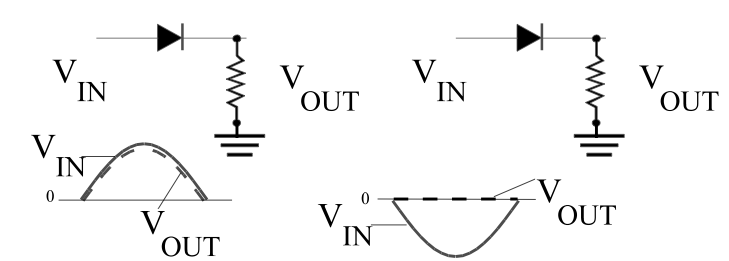
\includegraphics[width=\textwidth,trim=0 0 0 0,clip=false]{hwrectifier.png}
\caption*{Half-wave rectification.}
%\label{fig:1}
\end{center}
\end{figure}
\par Now about that ``slightly greater''... 
If we continue the one-valve analogy real diodes are like spring loaded valves; 
in order to open the valve to allow flow, a small amount of pressure is needed to overcome the spring resistance. 
This results in a fixed pressure drop across the valve. 
In the diode this loss of potential energy is a voltage called the ``turn on voltage'' or $V_{TO}$ and it is dependent on what the diode is made of. 
Silicon diodes have a $V_{TO}$ of 0.7 volts, germanium diodes have a $V_{TO}$ of 0.3 volts and most LEDs (Light emitting diodes) have a $V_{TO}$ of 1.3 volts. 
For the purposes of this class unless you are told otherwise we'll assume silicon diodes.

\par If you want a constant 0.7 volts source, the circuit below can do it for you. As long as $V_{IN}$ is  $> 0.7$ volts, $V_{OUT}$ = 0.7 volts.
\begin{figure}[!ht]
\begin{center}
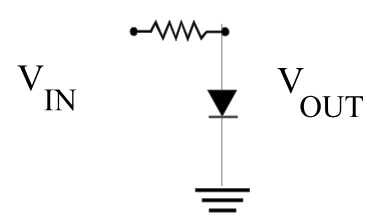
\includegraphics[width=0.25\textwidth,trim=0 0 0 0,clip=false]{diodesource.png}
\caption*{Diode voltage source.}
\end{center}
\end{figure}
\par However, 0.7 volts isn't particularly useful. Wouldn't it be handy to be able to create other constant voltage sources as easily? Enter the Zener diode.
A Zener diode (drawn as below) acts just like a regular diode in the forward direction. 
If $V_A > V_B$, current can flow through the diode with a $V_{TO}$ of 0.7 volts. 
Where the Zener diverges from conventional diodes is in the reverse direction. 
If $V_B > V_A$ no current flows until $V_B + V_Z = V_A$, where $V_Z$ is the Zener voltage.
The Zener can be thought of as a pair of diodes connected as below, where diode X has a $V_{TO}$ of 0.7 volts and diode Y has a $V_{TO}$ of $V_Z$.
\begin{figure}[!ht]
\begin{center}
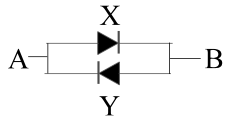
\includegraphics[width=0.25\textwidth,trim=0 0 0 0,clip=false]{zener.png}
\caption*{Zener diode equivalent circuit.}
\end{center}
\end{figure}

{\bf Task 4: LED circuit}\\
Build the circuit shown below on a breadboard using an LED.
Note that the exact value of the resistor may change subject to parts availability.
First, use the DC power supply to place a constant voltage between the input and ground. 
Start with the power supply at 0 V and slowly increase the voltage.
Now reverse the polarity of the LED, and note that it only turns on in one orientation.
Then, disconnect the power supply and connect the signal generator in its place. 
Connect an oscilloscope across the diode to see the voltage across it.
Set the signal generator to produce a 5 Hz sinusoid, and vary the amplitude of the signal. 
The LED will blink.
What happens as the signal amplitude increases? Why? Which parts of the signal correspond to the time when the LED is on?
Now place the oscilloscope leads across the resistor. What do you see? \underline{Show the TA your circuit and results.}
\begin{figure}[!ht]
\begin{center}
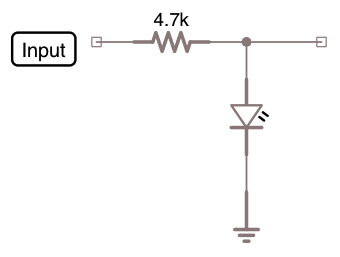
\includegraphics[width=0.4\textwidth,trim=0 0 0 0,clip=false]{ledcircuit.png}
\caption*{LED circuit to build.}
\end{center}
\end{figure}

{\bf Digital Circuits}\\
The dominant two types of digital circuits are TTL and CMOS. 
TTL stands for Transistor-Transistor Logic and CMOS for Complementary Metal Oxide Semiconductor. 
TTL runs on 5 volt power, (labeled Vcc for reasons known only to Sparky, god of power supplies) is generally faster than CMOS and consumes much more power. 
CMOS has flexible (3 to 12 volt) power needs and consumes much less power (making it ideal for battery-powered devices) but it is generally slower than the equivalent TTL chip. 
Recent advances in a 3 volt TTL technology is reducing some of the drawbacks to TTL. 
Digital circuits have the property of having binary states, that is they are either on (a digital 1) or off (a digital 0). 
For digital chips to ``talk'' to each other there has to be an agreement as to what represents a one and what represents a zero.
\begin{figure}[!ht]
\begin{center}
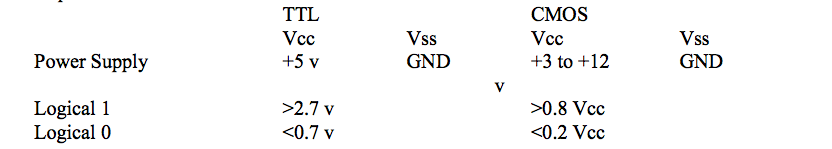
\includegraphics[width=\textwidth,trim=0 0 0 0,clip=false]{logicvoltages.png}
%\caption*{LED circuit to build.}
\end{center}
\end{figure}

{\bf NOT, AND, OR, EXOR}\\
The simplest logical function is the NOT function or inverter. 
Whatever logical state (1 or 0) is applied to the input, the opposite state is created on the output.
\begin{figure}[!ht]
\begin{center}
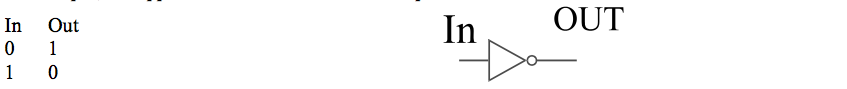
\includegraphics[width=\textwidth,trim=0 0 0 0,clip=false]{not.png}
%\caption*{LED circuit to build.}
\end{center}
\end{figure}
\par The next two most simple logic gates are the AND function and the OR function. 
These two both take two input to determine an output. 
With the AND function if A and B are 1 then Out is 1.
\begin{figure}[!ht]
\begin{center}
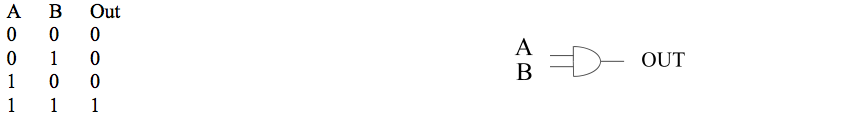
\includegraphics[width=\textwidth,trim=0 0 0 0,clip=false]{and.png}
%\caption*{LED circuit to build.}
\end{center}
\end{figure}
\par The OR function produces a 1 if A or B are 1.
\begin{figure}[!ht]
\begin{center}
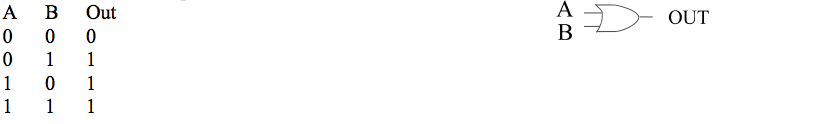
\includegraphics[width=\textwidth,trim=0 0 0 0,clip=false]{or.png}
%\caption*{LED circuit to build.}
\end{center}
\end{figure}
\par Finally there is an Exclusive OR function. Called EXOR or the difference function, it produces a 1 when A or B are high but not both. This can also be described as exerting a 1 when A differs from B.
\begin{figure}[!ht]
\begin{center}
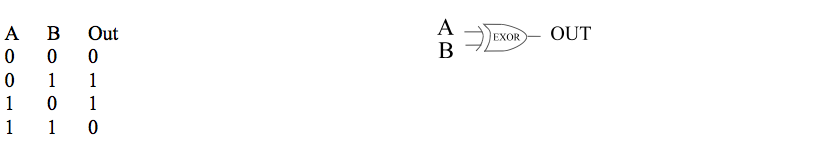
\includegraphics[width=\textwidth,trim=0 0 0 0,clip=false]{exor.png}
%\caption*{LED circuit to build.}
\end{center}
\end{figure}
\pagebreak
\par Given that both the inputs and outputs can only be one or zero, what's all the hoopla about digital logic? 
Well, binary arithmetic is the engine behind computers and we can use basic logic functions to create mathematical functions such as addition and subtraction but there is the issue of time. 
A square wave can be thought of as a train of ones and zeros.
\begin{figure}[!ht]
\begin{center}
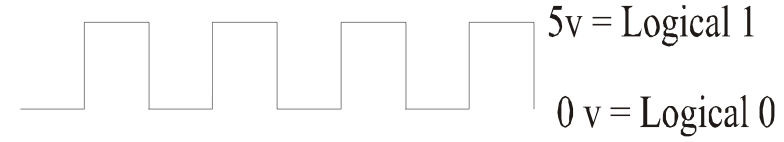
\includegraphics[width=\textwidth,trim=0 0 0 0,clip=false]{squarewave.png}
\caption*{Square wave.}
\end{center}
\end{figure}

\par Logic chips as well as analog integrated circuits are available in a number of forms. 
While the demand for smaller and smaller sizes is increasing the use of surface mount chips, for the lab we will use chips in a format called Dual Inline Package or DIPs. 
This chip format consists for two parallel sets of pins on each side of a rectangular chip. 
The standard packages are 8 pin (op amps and some oscillators), 14 pin (logic and oneshots), 16 pin (counters and some logic), 22 pin and a few larger sizes for things like memory chips and old style CPUÕs.

\par In Data Books you find which function is performed by each of the chipsÕ pins. 
An example of a Data sheet is attached to this lab. 
The pin numbers of the chips are shown below. 
There is generally a notch or dip telling you which pin is \#1. 
Look for this since
occasionally the lettering on top of the chip is upside down.
\begin{figure}[!ht]
\begin{center}
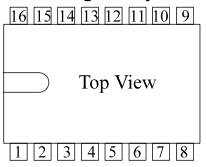
\includegraphics[width=0.25\textwidth,trim=0 0 0 0,clip=false]{dip.png}
\caption*{Notched chip.}
\end{center}
\end{figure}

%\item{\bf Construction tips}\\
%How do you move from a breadboarded lab circuit to a stand-alone device?
%Analyze what you need in terms of inputs, outputs, power. 
%Construct prototypes of subsections and test them individually. 
%As the prototypes work, you may want to move them to some semi-permanent form. 
%I generally go from breadboard to wirewrap. 
%If the wirewrapped circuits perform as I want them to I may add some solder to the wrapped connections to make them more stable.
%
%\par Once the circuit is doing what I want, how is it going to be powered? 
%Batteries, power supply? 
%Can I put the power supply in the box with the circuit? 
%How am I going to get signals into and out of the box? 
%How much flexibility of connections do I need? 
%You should do all of these things before you even look at boxes.
%\par Rule of Thumb: ``Putting something in a box doubles the project time.''
%Tips: 1) Power supply lines going through boxes (especially metal boxes) should have a grommet. 
%2) You can never have too many capacitors on your power supply lines.

\end{enumerate}

\newpage

\noindent Parts List:\\[0.2em]
\begin{tabular}{|r|l|}
\hline
2.7 k$\Omega$ Resistor & 1 \\ \hline
4.7 nF Capacitor & 1 \\ \hline
Breadboard & 1 \\ \hline
Wire & \\ \hline
4.7 k$\Omega$ Resistor & 1 \\ \hline
LED & 1 \\ \hline
Assorted Resistors & 10 \\ \hline
Solder & 1 Spool \\ \hline
DIP chip & 4 \\ \hline
Wick & 1 \\ \hline
Plated perfboard & 1 \\ \hline
Plain perfboard & 1 \\ \hline
\end{tabular}

\end{document} 